\section{Evaluation}\label{sec:evaluation}
This section reports what the precompile-enabled zkVM regime can and cannot do for PLUM-based BDEC on consumer hardware, and reads the measurements back against the cost framework of Section~\ref{sec:theoretical}. Four findings answer the thesis's question, one per contribution. \emph{Feasibility}: the Griffin precompile turns PLUM verification from a non-terminating run into a $14.24$-minute proof within the $24$~GB envelope (Table~\ref{tab:plum-verify}). \emph{The cost criterion}: that precompiled hash nonetheless proves slower than a software SHA-3 control ($14.24$ versus $13.24$~min), an inversion whose sign the trace-area model postdicts. The measured evidence gives three results (the design-level field-multiplication verdict is Section~\ref{sec:system}'s). Griffin removes $58.5\times$ cycles yet loses on committed area. The matched-field control confirms the necessity direction ($164\times$ tax, execute mode). The power-residue symbol pays $10.33\times$ on total committed area (\S\ref{ssec:attribution}, \S\ref{sssec:already-served}). \emph{The credential characterisation}: both credential relations run and prove on SP1 (Table~\ref{tab:bdec}). \emph{The dual obstruction}: the zero-knowledge wrap completes in $46.83$~minutes but is pairing-based and so classical, not post-quantum (\S\ref{ssec:resource-frontier}). Within the scope of the literature we surveyed these are among the first such figures; the configurations that do not complete are reported alongside those that do, and everything that follows is the evidence for these four.

\subsection{Setup and Methodology}\label{ssec:eq}
We measure PLUM verification and the credential relations built on it with and without the precompile suite, attribute where the zkVM cost falls and how much the suite removes, locate the resource boundary for the configurations that do not complete, and compare the zkVM and static-circuit regimes on update churn (Definition~\ref{def:update-churn}).

\paragraph{Two measurement modes.}
\emph{Execute mode} counts RISC-V cycles without producing a proof; its cost is machine-independent and always terminates. \emph{Prove mode} produces the receipt, is the deployment-relevant cost, and does not always complete on the target hardware. We therefore report prove wall-clock where proving completes and fall back to execute-mode cycles where it does not, never comparing the two across that boundary; each table states its mode. \emph{Feasible} means the prove completes within the $24$~GB envelope; whether a completed time is \emph{acceptable} is a separate judgment this chapter does not make: the deployment trade-offs it turns on are weighed in Section~\ref{sec:discussion}, and the operational bar the thesis does and does not state is fixed in Section~\ref{sec:conclusion}.

\paragraph{What we do not claim.}
We report no single ``$N\times$ speedup.'' The with/without-precompile contrast at the prove level is an \emph{infeasible-to-feasible} transition, not a ratio of two finite times (\S\ref{ssec:headline}); the finite reductions we report are cycle-level, at a stated security level and mode.

\paragraph{Platform.}
Table~\ref{tab:platform} lists the evaluation platform; all prove-mode measurements are local single-machine runs with no network or dev-mode acceleration unless stated.

\begin{table}[H]
\centering
\small
\begin{tabular}{ll}
\toprule
Component & Specification \\
\midrule
Hardware & Apple M5~Pro, 18-core CPU, 20-core GPU, 24~GB unified memory, 1~TB SSD \\
OS & macOS 26.5 (Darwin 25.5.0), Apple Silicon (arm64) \\
Prover & CPU-bound; no CUDA/network prover (Apple Silicon has no NVIDIA GPU path) \\
zkVM & SP1 v6.2.1 (forked) \\
Signature & PLUM over $\mathbb{F}_p$, $p=2^{64}p_0+1$ ($199$-bit; see \S\ref{ssec:bigint}) \\
Security levels & $\lambda=80$ (prove-mode runs; Griffin-delta and credential execute figures), $\lambda=128$ (cost-attribution analysis, \S\ref{ssec:attribution}) \\
\bottomrule
\end{tabular}
\caption{Evaluation platform and measurement setup.}
\label{tab:platform}
\end{table}

\subsubsection{Settings Justification}\label{ssec:settings-justify}
Each fixed parameter is one a deployer would plausibly choose; we disclose where a setting is tuned.

\begin{description}
  \item[Consumer hardware (M5~Pro, 24~GB).] The research question concerns deployability on a personal machine, so this hardware is the thesis's explicit scope. Every feasibility claim is scoped to this envelope and is not asserted in general.
  \item[Security level: $\lambda=80$ for prove-mode, $\lambda=128$ for cycle attribution.] We disclose this seam. Prove-mode runs use $\lambda=80$ because $\lambda=128$ proving is untested and expected to exceed the memory budget, the precompile-free arm already failing at $\lambda=80$ (Table~\ref{tab:plum-verify}). $\lambda=80$ is the largest level at which prove-mode wall-clock is observable on this hardware, which is why we use it and not because it is favourable. The cost-attribution analysis (\S\ref{ssec:attribution}) is reported at the audience-relevant $\lambda=128$ because it is machine-independent (execute mode) and so remains measurable where proving is not. No number mixes the two levels silently. Each table states $\lambda$.
  \item[Prover memory tuning.] At SP1's default settings the Cell~2 prove is OOM-killed after ${\approx}3$~min on the $24$~GB machine. A documented reduced-memory configuration (\texttt{SHARD\_SIZE}$\,=2^{22}$, default $2^{24}$; \texttt{ELEMENT\_THRESHOLD}$\,=2^{26}$; \texttt{HEIGHT\_THRESHOLD}$\,=2^{20}$; \texttt{TRACE\_CHUNK\_SLOTS}$\,=2$; \texttt{RAYON\_NUM\_THREADS}$\,=8$, default $18$; \S\ref{ssec:repro}) trades smaller, more numerous shards and fewer threads for fitting the envelope, so the headline timings are tuned-configuration times (Cell~2 $14.24$~min, SHA-3 control $13.24$~min under identical tuning; the zero-knowledge wrap ${\approx}15$~GiB peak, \S\ref{ssec:resource-frontier}). One contributing factor to the Griffin arm's memory pressure: the fork's shard-budgeting table prices the Griffin chip at $348$ trace columns against its compiled $3{,}819$, so a Griffin-bearing shard is budgeted at roughly a tenth of its committed area and split later than the trace-area threshold intends; correcting the entry is a one-line change whose effect on Cell~2 is untested and left to future work.
  \item[Micro-benchmark isolation.] Cost-attribution runs isolate single primitives (one Griffin permutation; one verification) so that per-operation cost can be attributed rather than inferred from an aggregate.
\end{description}

\subsubsection{Reproducibility}\label{ssec:repro}
Prove-mode and attribution runs use fixed RNG seeds and fixed messages. The SP1 submodule version is pinned in the lockfile. The memory-tuning environment variables, host binaries, and the adversarial-probe harness are recorded in the project's measurement notes, together with the per-run commit hashes and, where applicable, guest-image identifiers. The exception is an earlier, retired pair of CreGen prove runs (the $26.98$/$27.45$~min pair; \S\ref{ssec:frontier}): their shard configuration was recorded only in a human-written summary rather than machine-echoed in the run log, and does not reproduce on the shipped fork. The credential-relation prove figures of Table~\ref{tab:bdec} are the config-verified runs of \S\ref{ssec:frontier}.

\subsection{PLUM Verification With and Without the Precompile}\label{ssec:headline}

Table~\ref{tab:plum-verify} reports prove-mode results for a single PLUM signature verification at $\lambda=80$. The central comparison is between the precompile-free baseline and the precompile-enabled arm on the same hardware. Its rows label Cell~1/2/3 as no precompile / Griffin precompile / SHA-3 control, and the control is not a deployable variant.

\begin{table}[H]
\centering
\small
\begin{tabular}{lllll}
\toprule
zkVM / mechanism & $\lambda$ & Prove time & Peak mem & Outcome \\
\midrule
Cell~1: SP1, rv64im Griffin (no precompile)  & 80 & n/a       & ${\approx}13.6$~GiB & DNF (stopped at $5$\,h\,$07$\,m) \\ % Cell 1 tuned; master_batch_20260706 C1e (watchdog 1200s cap, peak 13.62 GB, well under 24 GB)
\textbf{Cell~2: SP1, Griffin-$\mathbb{F}_p^{192}$ precompile (this work)} & \textbf{80} & \textbf{14.24~min}\textsuperscript{\dag} & \textbf{${\approx}13.7$~GiB} & \textbf{receipt verified} \\          % 582ad1a Cell 2 (this work, emphasized); n=5 master_batch_20260706
Cell~3: SP1, SHA-3 hasher (control)          & 80 & 13.24~min\textsuperscript{\dag} & ${\approx}14.4$~GiB & receipt verified \\ % 91941ed; n=5 master_batch_20260706
\bottomrule
\end{tabular}
\caption{PLUM verification, prove mode ($\lambda=80$; the Griffin instance runs at $14$ rounds, one below the security-conservative $15$ of Table~\ref{tab:round-margin}).}
\label{tab:plum-verify}
\end{table}

A run of the precompile-free arm under the documented reduced-memory tuning (\S\ref{ssec:settings-justify}) ran for $5$\,h\,$07$\,m without terminating and without exhausting memory before we stopped it by hand, yielding no receipt. Under that tuning the binding resource is time rather than memory, and the prove still does not complete within five hours on this hardware.

\paragraph{The honest reading.}
The with/without-precompile contrast is not a ratio of two finite times. Without the precompile the workload \emph{does not complete} on this hardware, and with it the workload completes in $14.24$~minutes (mean of five runs, $14.16$--$14.44$). The defensible claim is therefore qualitative at the prove level (\emph{the precompile moves PLUM verification from infeasible to feasible on consumer hardware}) and quantitative only at the cycle level (\S\ref{ssec:attribution}).

The SHA-3 control does not isolate the hash family (it differs from the Griffin arm in two things at once, the hash (bit-oriented SHA-3 against $\mathbb{F}_p^{192}$ Griffin) and the field, matched only on the security level $\lambda$, so it is a deliberately confounded control rather than a hand-picked favourable setting). The verification harness is identical except that every Griffin-$\mathbb{F}_p^{192}$ sponge call is replaced by a SHA3-256 call computed in software, so that the SHA-3 arm fires \emph{no} hash precompile and only the shared \texttt{UINT256\_MUL} field-multiplication precompile remains active. It shows that a workload using a \emph{standard} hash in software is cheaper, by the margin the next paragraph quantifies, than one using the algebraic hash PLUM requires through a bespoke chip, which is the quantitative form of the field-mismatch-tax argument of Section~\ref{sec:theoretical}.

The inversion is direct. The bespoke Griffin-$\mathbb{F}_p^{192}$ precompile proves \emph{slower} at prove than the software SHA-3 control at matched $\lambda=80$ in every run we took. The sign is robust. At a fixed tuned config on a clean machine, five Cell~2 runs and five Cell~3 runs give means of $14.24$~min (range $14.16$--$14.44$) and $13.24$~min (range $13.02$--$13.38$), a magnitude of ${\approx}1.08\times$ in wall-clock and ${\approx}1.11\times$ in cycles, with each arm's prove-time spread under $5\%$. An earlier single run measured $32.53$ versus $13.28$~min; its high Cell~2 figure was not reproduced under fixed-config replication and is attributed to machine-state contamination rather than an intrinsic build difference, so the reported value is the replicated $14.24$~min.

\paragraph{Why the model postdicts the sign.}
We read the inversion as a genuine property of the pipeline rather than a measurement artefact, and the trace-area accounting of Section~\ref{sec:theoretical} (Equation~\eqref{eq:trace-area-model}) postdicts its sign from the chips' committed dimensions. The Griffin chip emits $14$ rows of $3{,}819$ columns per permutation (each row carries $26$ modular-arithmetic gadgets of $127$ cells each, beside range checks and state limbs), so the $1{,}052$ permutations of one verification commit $14\times 3{,}819\times 1{,}052\approx 5.6\times10^{7}$ cells, plus one controller row per permutation, that the SHA-3 arm never pays. The shared \texttt{UINT256\_MUL} chip is common-mode ($69{,}396$ versus $69{,}385$ events) and cancels, and the Griffin arm additionally executes $11\%$ more guest cycles ($1.23\times10^{8}$ versus $1.11\times10^{8}$, execute mode). Both terms of Equation~\eqref{eq:trace-area-model} are therefore larger on the Griffin arm, so the model places it behind the control for every non-negative choice of the per-cell rates, granted a common per-cycle core area across the two arms. The calibration of the model's constants on these two arms is reported with the cost model (\S\ref{ssec:costmodel}). The feasibility recovery and the inversion are the same cost model (Equation~\eqref{eq:trace-area-model}) evaluated at two operating points. With the precompile the run completes and can be measured, and the cost model explains why it is still no faster than the control. The control's hash costs the substrate no chip area at all, while the Griffin arm pays for its chip and saves nothing in return.

Not all of that width is irreducible. Of the twenty-six field operations per row, about ten are genuine $192$-bit multiplications, the S-box arithmetic that no small field avoids. The other sixteen are additions and small linear combinations. They are charged at the full multiplication price only because the chip reuses one circuit for both, so a dedicated addition path would cut about a quarter of each row. Even so trimmed, every remaining cell still computes over the $199$-bit field, so a leaner chip narrows the gap toward parity but does not reverse its sign against a hash whose cost is field-invariant.

The inversion is moreover conservative twice over. The SHA-3 control runs in software with no chip of its own, so a native bit-hash precompile would only widen the gap, and the Griffin instance is arithmetised at $14$ rounds against the $15$ its parameters call for (Section~\ref{sec:security}, Table~\ref{tab:round-margin}), so a correctly-secure instance adds roughly another fourteenth of the Griffin cells and widens the gap further.

\paragraph{Proof size, and the wrap that produces it.}
Receipt size in SP1 is a property of the proof \emph{type}, not of the workload. The runs above use SP1's default \emph{core} proof, whose size \emph{scales with execution size}~\cite{succinct2025prooftypes}. The compact, on-chain-deployable proof is instead the constant-size {SNARK} \emph{wrap} of that receipt, about $260$~bytes for Groth16 over {BN254}, or $868$~bytes for {PLONK}~\cite{succinct2025prooftypes}. Producing that wrap completes on the target hardware: the full sound {PLONK}/{BN254} chain wraps one PLUM verification into a verified constant-size proof in $46.83$~minutes at a $15.29$~GiB peak, inside the $24$~GB budget and without the default path's multi-day regeneration (\S\ref{ssec:resource-frontier}). On a $24$~GB machine the deployer can therefore generate either the large, shard-scaling core receipt or the $260$-to-$868$-byte {SNARK} wrap of it; the post-quantum gap that wrap leaves is taken up in \S\ref{ssec:resource-frontier}. We report the wrapped figure as measured and do not serialise the workload-dependent core receipt, whose byte count is not the deployment-relevant number.

\paragraph{An empirical witness leak on the non-zero-knowledge core path.}
The core receipt's workload-dependence is not merely formal. Fixing the relation and varying only the witness across $N=20$ standalone PLUM verifications, the Griffin permutation count is witness-invariant at $1{,}052$, while the field-multiplication count and the total cycle count vary from witness to witness (execute mode). The variation reaches the verifier-observable proof. Three prove-mode runs on distinct witnesses ($N=3$) produce core receipts of $154.67$, $156.12$, and $153.21$~MB, all distinct, a ${\approx}1.9\%$ spread. Because the shipped core STARK is not zero-knowledge (\S\ref{ssec:resource-frontier}), this leak is on a path where no anonymity is claimed. A constant-size zero-knowledge SNARK wrap removes it, its byte count being independent of the witness (about $260$~bytes for Groth16 over BN254, $868$ for PLONK; Figure~\ref{fig:proof-collapse}). That wrap completes on this hardware (\S\ref{ssec:resource-frontier}), so on the wrapped path the leak closes. What it does not close is post-quantum security, because that wrap rests on a {BN254} pairing (\S\ref{ssec:resource-frontier}): the leak's fix and the anonymity gap are the same wrap seen from two sides.

\begin{figure}[H]
\centering
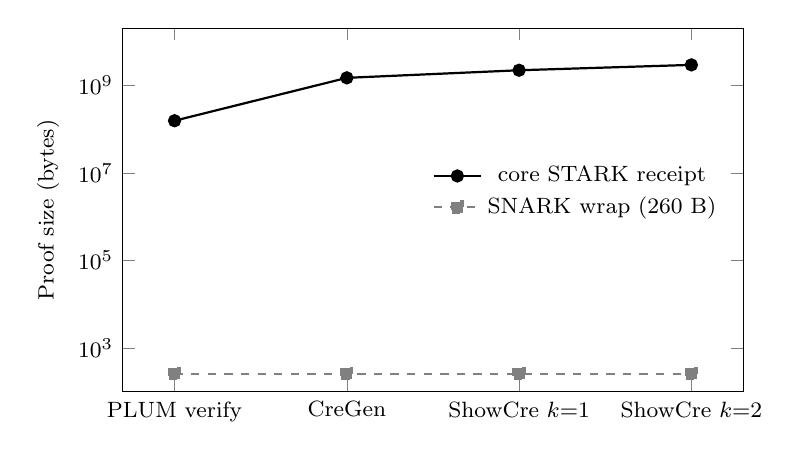
\begin{tikzpicture}
\begin{axis}[
  width=0.78\textwidth, height=6.2cm,
  ymode=log, log basis y={10},
  ylabel={Proof size (bytes)},
  symbolic x coords={PLUM verify, CreGen, ShowCre $k{=}1$, ShowCre $k{=}2$},
  xtick=data,
  ymin=1e2, ymax=2e10,
  tick label style={font=\footnotesize}, label style={font=\footnotesize},
  x tick label style={font=\footnotesize},
  legend style={font=\footnotesize, at={(0.98,0.55)}, anchor=east, draw=none, fill=none},
  clip=false,
]
\addplot[mark=*, black, thick] coordinates {
  (PLUM verify, 154665328) (CreGen, 1473690434) (ShowCre $k{=}1$, 2195116844) (ShowCre $k{=}2$, 2911822343)
};
\addlegendentry{core STARK receipt}
\addplot[mark=square*, gray, dashed, thick] coordinates {
  (PLUM verify, 260) (CreGen, 260) (ShowCre $k{=}1$, 260) (ShowCre $k{=}2$, 260)
};
\addlegendentry{{SNARK} wrap ($260$~B)}
\end{axis}
\end{tikzpicture}
\caption{Within-pipeline proof-size collapse (same scheme, same runs).}
\label{fig:proof-collapse}
\end{figure}

\subsection{Cost Attribution}\label{ssec:attribution}
To attribute the cost we use execute-mode cycle counts at $\lambda=128$, the audience-relevant security level, where prove-mode is infeasible but cycle counts remain machine-independent. Table~\ref{tab:ablation} reports the cumulative effect of routing PLUM's field arithmetic through the host precompile, as an ablation over the SHA-3-hasher verification path.

\begin{table}[H]
\centering
\small
\begin{tabular}{lrr}
\toprule
Configuration (cumulative) & SP1 cycles & $\Delta$ vs.\ baseline \\
\midrule
Baseline (\texttt{BigUint} emulation)        & 289{,}778{,}709 & n/a \\
$+$ field mul via host precompile            & 276{,}643{,}994 & $-4.5\%$ \\
$+$ power as square-and-multiply             & 240{,}857{,}140 & $-16.9\%$ \\
$+$ skip redundant reduction                 & 179{,}952{,}920 & $-37.9\%$ \\
\bottomrule
\end{tabular}
\caption{Cycle-level cost attribution of the field-arithmetic optimizations.}
\label{tab:ablation}
\end{table}

\paragraph{Where the cost lives, and the parameter-set caveat.}
At $\lambda=128$ a single PLUM verification on the SHA-3-hasher arm issues about $112{,}902$ $\mathbb{F}_p^{192}$ multiplication syscalls through the host precompile, as counted in our own SP1 run log. No Griffin permutation executes on that arm, so this figure measures the verifier's \emph{non-hash} field arithmetic (PLUM \S4.2 reports $\approx 10^4$ non-hash algebraic R1CS constraints, $10{,}333$ of $116{,}285$). The Griffin-internal multiplication cost appears instead in the with/without-AIR contrast at $\lambda=80$. The software-Griffin arm fires $4{,}870{,}724$ \texttt{UINT256\_MUL} syscalls against $69{,}396$ with the Griffin AIR active, the hash-internal field operations either absorbed by the \texttt{GRIFFIN\_FP192\_PERMUTE} syscall or inflating the multiplication count $70\times$. The contrast is therefore consistent with the field-mismatch cost model. The cost is dominated by the algebraic hash, whose internal field operations leave the syscall stream only when the bespoke chip absorbs them. We caution explicitly against transferring the PLUM paper's circuit-SNARK figure (that $91\%$ of \emph{R1CS constraints} are hash work) directly to the zkVM cost model. That figure is a constraint count in a different proving system, whereas Table~\ref{tab:ablation} is a RISC-V cycle count. The qualitative conclusion (hash/field arithmetic dominates) agrees. The exact share differs by cost model and is reported here in the zkVM's own units.

\paragraph{Execute-mode delta for the Griffin precompile (PLUM-80).}
For the bespoke Griffin AIR specifically, the precompile-free versus precompile-enabled execute-mode cycle counts differ by a factor of $58.5\times$ at $\lambda=80$, the ratio of precompile-free to Griffin-AIR-enabled cycles on the Griffin arm. This is close to the field-mismatch tax of Proposition~\ref{prop:fmt-lb}. It exceeds the schoolbook $\ell^2\approx 49$ per-multiplication estimate because the whole Griffin permutation collapses into a single precompile call, rather than being emulated one multiplication at a time. This is distinct from the $37.9\%$ of Table~\ref{tab:ablation}, a separate field-multiplication-reduction ablation reported at $\lambda=128$. 
We report this as an \emph{execute-mode cycle ratio} rather than a wall-clock speedup. It is the machine-independent counterpart of the infeasible-to-feasible prove transition of Table~\ref{tab:plum-verify}, and it is the figure that should be cited when a single number is wanted, in place of any prove-time ``speedup,'' which is undefined when the baseline does not complete.

\subsection{The Credential Relations and the Consumer-Hardware Frontier}\label{ssec:frontier}
Moving from a single signature to the credential-generation relation $R_{\mathsf{cre}}^{\Sig}$ instantiated with PLUM (two signature verifications under a hidden user key; \S\ref{ssec:integration}), Table~\ref{tab:bdec} reports the application-level results at $\lambda=80$. These are execute-mode cycle counts and SP1 succinct-prove-mode wall-clock for both credential relations.

\begin{table}[H]
\centering
\small
\begin{tabular}{l l p{3.2cm} p{4.6cm}}
\toprule
Workload & Mode & Cost & Outcome \\
\midrule
CreGen & execute & $9.12\times10^{10}$ cyc & both verifications accept \\ % SP1 software-Griffin, sp1_bdec_execute_20260707 (91,177,673,619 cyc, standard-Griffin)
CreGen, SP1 & prove (succinct) & $68.96$~min ($1.47$~GB proof, $n{=}1$) & succinct receipt verified \\ % config-verified HEIGHT_THRESHOLD=2^16
ShowCre $k{=}1$, SP1 & prove & $103.34$~min ($2.2$~GB proof, $n{=}1$) & succinct receipt verified \\
ShowCre $k{=}2$, SP1 & prove (succinct) & $136.82$~min ($2.9$~GB proof, $n{=}1$) & succinct receipt verified \\
\bottomrule
\end{tabular}
\caption{Credential relations: execute and prove-mode cost ($\lambda=80$).}
\label{tab:bdec}
\end{table}

The execute-mode result validates the honest path of the BDEC credential relation end-to-end inside the zkVM. Both signature verifications accept, at $9.12\times10^{10}$ cycles. The CreGen prove figure of Table~\ref{tab:bdec} is the config-verified reproducible completing prove, $68.96$~min ($1.47$~GB proof) at \texttt{HEIGHT\_THRESHOLD}$=2^{16}$; an earlier $26.98$/$27.45$~min ($296$~MB proof) pair was faster but its shard configuration was recorded only in a human-written summary, not machine-echoed, and does not reproduce on the current fork, so it is not used. The ShowCre figures are likewise the config-verified reproducible completing proves at $k{=}1,2$. Rejection behaviour was probed only at single-verification scope (Section~\ref{sec:system}). On SP1 both credential relations complete a succinct (non-zero-knowledge) prove (Table~\ref{tab:bdec}); the credential-generation wrap and both the $k{=}1$ and $k{=}2$ showing wraps complete and verify within the memory budget, the $k{=}2$ wrap statement-bound.

\paragraph{Both relations bind their public statement.}
The proves of Table~\ref{tab:bdec} are outcome-only. A statement-bound variant additionally commits each relation's public statement to the receipt journal and recovers it on verification. A statement-bound CreGen prove completes in $66.05$~min, accepting, with the committed $x_{\mathsf{cre}}=(c,h,\mathsf{ppk})$ recovered and matched against the input; a full end-to-end run binds the showing as well, with two cross-issuer CreGen issuances ($66.14$ and $65.59$~min) and a $k{=}2$ ShowCre presentation ($127.94$~min) each accepting, its committed statement recovered and matched, the presentation binding $x_{\mathsf{show}}=((\mathsf{ppk}_{\mathsf{TA}})_j,\mathsf{ppk}_{UV},h_{UV})$ while keeping the shown credential private. Binding composes with the zero-knowledge wrap in a single run: a statement-bound CreGen wrap (the jbind guest of Section~\ref{sec:system} through the full chain of \S\ref{ssec:resource-frontier}) completes and verifies in $4.18$~h at a $15.2$~GiB peak, and the showing wrap likewise (the statement-bound $k{=}2$ figure in \S\ref{ssec:costmodel}), so both credential relations carry a measured statement-bound zero-knowledge wrap. The commitment cost is not separately resolvable: the bound CreGen prove ($66.05$~min) and wrap ($4.18$~h) each land within a few percent of their outcome-only counterparts ($68.96$~min, Table~\ref{tab:bdec}; $4.20$~h, \S\ref{ssec:resource-frontier}); both sides are single runs, so this is closeness between two runs rather than a variance-resolved bound, and binding is indistinguishable from free at single-run resolution.

\subsubsection{The post-quantum frontier}\label{ssec:resource-frontier}
The zero-knowledge wrap of a PLUM proof completes on the target hardware. The full sound chain (core, compress, shrink, wrap to {BN254}, and a native gnark {PLONK} proof of the fixed wrap circuit, with verifying-key verification on throughout) produces a verified constant-size proof of one PLUM single-signature verification (Cell~2 of Table~\ref{tab:plum-verify}, the $14.24$-min core prove) in $46.83$~minutes at a peak of $15.29$~GiB, inside the $24$~GB envelope with ${\approx}8.7$~GiB to spare. The credential relation wraps too. A full CreGen zero-knowledge wrap completes in $252$~minutes ($4.20$~h) at a $15.63$~GiB peak. Neither is memory-bound.

The wrap avoids the multi-day artifact regeneration the toolchain's default path implies. On the default path the wrap is killed at the recursive-compression step, because SP1's static recursion-shape and verifying-key tables are provisioned for smaller relations than PLUM verification, and rebuilding those tables in full is a one-time ${\approx}51$~h compute over $185{,}862$ entries (projected from a measured per-setup slope of ${\approx}1$~s across contiguous slices at the start, middle, and end of the table, \rr{docs/measurements/zkwrap_vkmap_slope_20260628}; the rebuild itself was never run, being exactly what the reduced table avoids). We circumvent that rebuild rather than pay it. The wrap verifies against a \emph{reduced} verifying-key table built from only the guest's own shard shapes ($19$ setups in $31$~s for PLUM verification, $26$ setups in $41$~s for CreGen) together with SP1's stock wrap circuit, which reuses the shipped {BN254} gnark circuit unchanged. The sound path is preserved (verifying-key verification stays on), so no recursion-shape rebuild and no circuit rebuild is needed. The gnark {PLONK} stage runs with its zero-knowledge blinding enabled, confirmed by a dedicated check in which two proofs of one witness differ under randomized blinding (\rr{docs/measurements/wrap_zk_check_20260707}). The pipeline's completion and its verifier acceptance are likewise measured. The post-quantum gap below holds independently of that check.

What the wrap does \emph{not} provide is post-quantum anonymity. The wrap rests on a {BN254} pairing, so the zero-knowledge it confers is classical-computational, sound against a classical distinguisher but not against a quantum one. A post-quantum-anonymous proof would need a post-quantum-sound recursive zero-knowledge wrap, which this toolchain does not offer. The provisioning wall therefore does not bind here; what does is the dual obstruction, whose analysis is Section~\ref{sec:security}'s and whose deployment reading is Section~\ref{sec:discussion}'s. The substrate can produce a zero-knowledge proof (over a classical pairing) or a post-quantum proof (the non-zero-knowledge core receipt), and not, as it ships, one proof that is both: the anonymity--deployability tension takes its measured form here.

A second and separate cost governs the wrap's \emph{wall-clock}, and it grows with the credential. The compress stage dominates the wrap tail and scales with the core proof's shard count. PLUM verification's $104$ shards compress in ${\approx}19$~min, whereas CreGen must be proved at \texttt{HEIGHT\_THRESHOLD}$=2^{16}$ to avoid a core-prove overflow, which splits it into $1{,}018$ shards and stretches the compress tail to ${\approx}166$~min (${\approx}0.16$~min per shard, near-linear). Peak memory stays bounded at ${\approx}15$~GiB throughout, so this is a time cost, not a memory cost. The BDEC wraps fit the $24$~GB envelope, but their wall grows about linearly with credential size, projecting past any practical bound for large disclosure sets (\S\ref{ssec:costmodel}). Memory is not the constraint here; the compress-tail cost is.

% \begin{figure}[H]
% \centering
% \begin{tikzpicture}
% \begin{axis}[
%   width=0.72\textwidth, height=6.2cm,
%   xlabel={Core-proof shard count}, ylabel={Compress-tail (min)},
%   xmin=0, xmax=1150, ymin=0, ymax=190,
%   xtick={0,104,1018}, xticklabels={$0$,$104$,$1{,}018$},
%   ytick={0,19,166},
%   tick label style={font=\footnotesize}, label style={font=\footnotesize},
%   clip=false,
% ]
% \addplot[dashed, gray, domain=0:1018, samples=2] {0.163*x};
% \addplot[only marks, mark=*, mark size=2.3pt, black] coordinates {(104,19) (1018,166)};
% \node[font=\footnotesize, anchor=north west] at (axis cs:135,24) {PLUM verify};
% \node[font=\footnotesize, anchor=south east] at (axis cs:1005,160) {CreGen};
% \node[gray, font=\footnotesize, anchor=south] at (axis cs:560,72) {${\approx}0.16$--$0.18$~min/shard};
% \end{axis}
% \end{tikzpicture}
% \caption{Compress-tail wall-clock against core-proof shard count.}
% \label{fig:compress-tail}
% \end{figure}

\paragraph{The precompile enlarges the recursion shape the wrap must verify.}
The default-path overflow, and the enlarged recursion shape the reduced verifying-key table must cover, attribute entirely to the Griffin-$\mathbb{F}_p^{192}$ precompile. Removing only the Griffin chip, with every other fork edit intact, reproduces the pre-Griffin compose shape byte-for-byte ($795{,}264$ provisioned ExtAlu events, md5 \texttt{f97a8b2f}). With the chip the provisioned shape is $1{,}072{,}032$, a marginal $+276{,}768$ ExtAlu ($+34.8\%$) and $+38{,}816$ PrefixSumChecks, while the fork's non-Griffin recursion edits move the shape by exactly zero. That enlargement (an actual required height of $1{,}064{,}022$, just under the provisioned shape, against the default $795{,}264$ budget) is what overflows the arity-$4$ compose shape on the default path, which is why the wrap is reached instead through a reduced table matched to the guest's own shard shapes. The precompile that lowers the core-layer cost is therefore the same chip that enlarges the recursion shape the wrap must verify, and hence the compress tail it must pay.

Separately, a \emph{non-zero-knowledge} baseline proof of a standardised-lattice signature verification (an ML-DSA proxy, the $17$ NTT-domain polynomial multiplications of $256$ coefficients modulo $q=8{,}380{,}417$ that dominate ML-DSA-65 verification, proved as a baseline succinct STARK on SP1, not a zero-knowledge wrap) was jetsam-killed after $249$~s with peak RSS $12.59$~GB and a virtual-memory footprint of $82.7$~GB (compressed memory plus swap, hence exceeding physical RAM). The measurement is a substrate base cost that \emph{strengthens but does not instantiate} the tension and supports the frontier claim, since it bears on the cost of proving any PQ verification on this substrate, not on the zero-knowledge wrap specifically. The positive feasibility anchors are the PLUM single-verification core prove of Table~\ref{tab:plum-verify} ($14.24$~min) and its zero-knowledge wrap ($46.83$~min, above). Table~\ref{tab:proof-mode} summarises, for every proof mode attempted, whether a receipt is produced and whether it is zero-knowledge and post-quantum.

\begin{table}[H]
\centering
\small
\renewcommand{\arraystretch}{1.2}
\begin{tabular}{@{}llccll@{}}
\toprule
Substrate & Configuration & ZK & PQ & Time & Peak \\
\midrule
SP1 & PLUM verify (core) & no & yes & $14.24$~min & --- \\
 & PLUM verify, SHA-3 (core) & no & yes & $13.24$~min & --- \\
 & PLUM verify, BN254 wrap & yes\textsuperscript{$\ddagger$} & \textbf{no} & $46.83$~min & $15.3$~GiB \\
 & CreGen (core) & no & yes & $68.96$~min & --- \\
 & CreGen, BN254 wrap & yes\textsuperscript{$\ddagger$} & \textbf{no} & $252$~min & $15.6$~GiB \\
 & ShowCre $k{=}1,2$ (core) & no & yes & $103$--$137$~min & --- \\
 & ShowCre $k{=}1$, BN254 wrap & yes\textsuperscript{$\ddagger$} & \textbf{no} & $706$~min\textsuperscript{$\P$} & $14.93$~GiB \\
Aurora & Loquat verify & no\textsuperscript{$\S$} & yes & $3.76$~min & --- \\
 & Loquat verify, ZK & yes & yes & ${\approx}22$~min ($n{=}3$) & --- \\
\bottomrule
\end{tabular}
\caption{Proof-mode feasibility: produced, zero-knowledge, post-quantum. \textsuperscript{$\ddagger$}~Zero-knowledge only over a {BN254} pairing (classical, not post-quantum); \textsuperscript{$\S$}~zero-knowledge supported for this circuit but disabled in this run; \textsuperscript{$\P$}~includes a one-time $2.96$~h core-shape pass (decomposition in \S\ref{ssec:costmodel}, where the statement-bound $k{=}2$ wrap, $10.21$~h, is also reported).}
\label{tab:proof-mode}
\end{table}

\subsection{Calibrating the Cost Model}\label{ssec:costmodel}
The cost criterion this chapter develops (\emph{when does a precompile pay?}) is decided on a single declared axis. The trace-area cost model of Section~\ref{sec:theoretical} (Equation~\eqref{eq:trace-area-model}) prices a primitive by the chip cells a precompile commits against the core cycles it removes, as a function of the field-mismatch width. We make that model the comparison axis explicitly, rather than comparing raw prove times across primitives, so that the matched and mismatched cases are commensurable on one quantity. The measurements above are point observations on this axis. To answer ``what would this cost at a configuration we did not run,'' we calibrate the model on them, validate it against the points we have, and state the prediction it makes for a point we have not yet run; the deployment decision this calibration feeds is taken up in Section~\ref{sec:discussion}. The model is fitted and validated in \emph{execute-mode cycle} counts. Carrying it to prove-mode wall-clock assumes the additive form survives recursion, memory pressure, segment aggregation, and the zero-knowledge wrap, any of which can introduce nonlinearity, so the prove-mode reading is an extrapolation, not a measured fit.

\subsubsection{Validation against the measured points}
The additive credential-cost model of Section~\ref{sec:theoretical} (Equation~\eqref{eq:cost-cregen}), linear in the per-verification cost $C_{\mathsf{ver}}$, is falsifiable against the two BDEC points we measured. The strongest internal check is CreGen. Equation~\eqref{eq:cost-cregen} predicts the two verifications should each cost $\approx C_{\mathsf{ver}}$ and together dominate the trace. The measurement bears this out directly. CreGen's software-Griffin execute cost is $9.12\times10^{10}$ cycles for its two verifications (Table~\ref{tab:bdec}), i.e.\ $\approx4.56\times10^{10}$ cycles per verification, and the per-verification cost holds to within $2\%$ across CreGen and both ShowCre instances (below), so the verifications account for essentially the whole CreGen trace and $C_0$ is small. For the Griffin hasher at $\lambda=80$, then, $C_{\mathsf{ver}}(\textsf{80},\textsf{Griffin})\approx 4.6\times10^{10}$ cycles. This per-verification figure counts a credential-relation verification, about $6{,}603$ Griffin permutations once the relation's Merkle and pseudonym hashing is included, larger than the $1{,}052$ of a standalone signature verification (Table~\ref{tab:plum-verify}), and consistent with it: both arms cost the same ${\approx}6.9\times10^{6}$ cycles per permutation ($4.56\times10^{10}/6{,}603$ here, $7.21\times10^{9}/1{,}052$ for the standalone arm below). We caution that this single relation validates the \emph{linearity} and the \emph{verification-dominance}, not the absolute constant at other $(\lambda,h)$. The $k=14$ projection below is labelled as such.

\paragraph{The hasher gap measures the tax.}
A single PLUM verification is markedly cheaper with the SHA-3 hasher control than with the Griffin algebraic hash, an order-of-magnitude separation that is the field-mismatch tax of Section~\ref{sec:theoretical} quantified at the verification level. Matched-$\lambda$ figures exist on SP1. At $\lambda=80$ in execute mode, at matched standalone single-verification scope ($1{,}052$ Griffin permutations, execute mode), the software-Griffin verification (Cell~1, no precompile) costs $7.21\times10^{9}$ cycles against $1.11\times10^{8}$ for the SHA-3 control (Cell~3), an order-of-magnitude (${\approx}65\times$) separation; the credential-relation per-verification figure of $4.56\times10^{10}$ cycles is larger only because it counts $6{,}603$ permutations and is not the matched comparison. The qualitative conclusion (that the algebraic hash is the tax-bearing component while the field arithmetic is not, so $C_{\mathsf{ver}}$ must be reported per hasher) holds regardless of the exact multiplier. The precompile narrows this gap (Table~\ref{tab:ablation}). Closing it entirely is what a native Griffin AIR on the proving path would buy.

\paragraph{ShowCre execute-mode cost (measured at $k=1,2$).}
The ShowCre relation is realised by the guest \texttt{bdec\_showcre\_plum\_griffin}, the $k+2$ generalisation of the CreGen guest, and measured in execute mode at the two running examples. At $k=1$ (the $\phi_1$ workload) ShowCre executes in $1.36\times10^{11}$ cycles, and at $k=2$ (the $\phi_2$ workload) in $1.82\times10^{11}$ cycles, each with all $k+2$ verifications accepting. Both agree with Equation~\eqref{eq:cost-showcre} at $C_{\mathsf{ver}}(\textsf{80},\textsf{Griffin})\approx 4.6\times10^{10}$. The per-verification cost is constant at $\approx 4.6\times10^{10}$ cycles across CreGen and both ShowCre instances (spread under $2\%$), so the additive $(k+2)\,C_{\mathsf{ver}}$ form is measured rather than assumed. Applying the same measured constant to a stress-test disclosure-set size, well beyond the running examples ($k=1,2$) and the $k\le 4$ design target, projects $\approx 7.3\times10^{11}$ cycles at $k=14$. A direct $k=14$ execute run does not reach this projection. The $16$ accumulated verifications exhaust the guest's default non-reclaiming bump allocator before the cycle count completes, an in-guest memory limit distinct from the prover-side wrap cost of \S\ref{ssec:resource-frontier} and clearable only by the reclaiming allocator at additional cycle cost. The $k=1$ and $k=2$ executions are correct and their cost is measured. The zero-knowledge \emph{proof} runs through the same wrap pipeline that completes for PLUM verification and CreGen (\S\ref{ssec:resource-frontier}). The $k=1$ wrap completes and verifies on the target hardware in $11.76$~hours end-to-end ($8.79$~hours for the per-proof wrap chain plus a one-time $2.96$~hour core-shape pass) at a $14.93$~GiB peak, within the $24$~GB envelope. The $k=2$ wrap likewise completes and verifies, and is statement-bound (the jbind guest of Section~\ref{sec:system} put through the same chain): $10.21$~hours end-to-end ($7.91$~hours for the per-proof wrap chain plus a one-time $2.30$~hour core-shape pass) at a $15.66$~GiB peak, again within the envelope. Across the two runs the quantities that grow with the verification count are the core-proof shard count ($1516$ at $k=1$, $2011$ at $k=2$) and the peak memory ($14.93\rightarrow15.66$~GiB), both staying within the budget; these are the config-stable readings of the compress-dominated model. The per-proof wall-clock is a single-run figure, not controlled for machine state across the two runs (see the thermal-throttling limitation below), so we rest the growth-in-$k$ statement on shard count and peak memory rather than on wall-clock. As with those workloads, the wrap it produces is zero-knowledge only over a {BN254} pairing (\S\ref{ssec:resource-frontier}).

\paragraph{Calibrating the trace-area constants.}
The trace-area model carries two constants. On the replicated runs of Table~\ref{tab:plum-verify} (Cell~2 Griffin $14.24$~min, Cell~3 SHA-3 $13.24$~min; \S\ref{ssec:headline}) the Griffin arm's prove-time residual over the control is only about a minute, too small to pin a positive per-cell rate against the chip's $5.6\times10^{7}$ cells, so the additive prove-time decomposition is near-degenerate on the trustworthy data. We therefore report an \emph{illustrative} calibration on an earlier run pair whose Cell~2 is the $32.53$-minute figure not reproduced under replication (\S\ref{ssec:headline}): there the control prices core work at $\kappa_{\mathsf{core}}\,\bar a_{\mathsf{core}}\approx 7.2\,\mu\mathrm{s}$ per guest cycle, and attributing the Griffin arm's residual $17.5$~minutes to its $5.6\times10^{7}$ cells gives $\kappa_{\mathsf{Griffin}}\approx 19\,\mu\mathrm{s}$ per committed cell (about $2.6$ guest cycles bought per committed cell). This magnitude is illustrative only, and nothing downstream rests on it. The model's out-of-fit content is the \emph{sign}, which is fixed by the committed cell and execute-mode cycle counts of \S\ref{ssec:headline} ($5.6\times10^{7}$ Griffin cells and $11\%$ more guest cycles, both machine-independent), and is therefore unaffected by the retired pair. Those orderings are consistent with the rest of Table~\ref{tab:plum-verify}. The precompile-free baseline's $7.21\times10^{9}$ cycles price at upwards of $14$~hours of core work alone (before the chip area of its $4{,}870{,}724$ \texttt{UINT256\_MUL} events is charged), consistent with its DNF, and against that baseline the precompile still pays by orders of magnitude, removing about $6.6\times10^{6}$ cycles per permutation against $5.3\times10^{4}$ cells added.

\paragraph{A deductive forecast: the matched-field point.}
The illustrative calibration above fixes two constants, both on the \emph{mismatched} side of the axis, where the primitive's native field ($199$ bits) is far wider than the prover's ($31$ bits). The model's out-of-fit content is the prediction it makes for a \emph{matched-field} operating point, at which a primitive native to the prover field needs essentially one limb, so a precompile commits chip area without removing a comparable multi-limb emulation from the core. On that point the precompile-pays inequality (Proposition~\ref{prop:precompile-pays}, Equation~\eqref{eq:precompile-pays}) predicts the precompile does \emph{not} pay. The removed core area shrinks toward zero while the added chip area does not, so the sign that the mismatched measurements postdict should \emph{reverse}. This forecast is, however, a \emph{deductive} consequence of the trace-area model rather than an independent test of it. As $\ell\to1$ the removed core area shrinks toward a single native operation while the added chip area does not, so the model cannot but predict no-pay there. An independent, out-of-sample test needs an operating point the two-constant calibration did not fix, and within PLUM that point is the already-served \texttt{FP192\_POW\_RES} break-even (\S\ref{sssec:already-served}), a large-prime chip on the construction's own primitive whose verdict the model forecasts and whose deciding measurement we specify there. A matched-field ($\ell=1$) point would be a further test, but every primitive in PLUM is $\ell=7$, so carrying it in prove mode would require building and proving a chip for an operation outside the construction, which we do not do; the execute-mode necessity test of the next subsection needs no chip and does use an out-of-construction $\ell=1$ multiplication. We therefore report the criterion as \emph{postdictive} on its two calibration points, with its out-of-fit content deductive at $\ell=1$ and tested at the \texttt{FP192\_POW\_RES} point, where the measured pay decides the forecast in its favour (\S\ref{sssec:already-served}).

\subsubsection{Matched-field control}
Distinct from the deductive matched-field forecast above (the keystone control of Section~\ref{sec:theoretical}, now a deductive consequence of the model), the necessity claim of the criterion (Proposition~\ref{prop:field-match}), that the field-mismatch benefit scales with the width $\ell$ and vanishes at $\ell=1$, admits a direct execute-mode test, forecast before the run (\rr{docs/measurements/keystone_matched_field_20260701}). We measure the per-multiplication emulated cost of a field-matched primitive (a KoalaBear single-limb multiplication, $\ell=1$, native to the prover field) against the mismatched $\mathbb{F}_p^{192}$ software multiplication ($\ell=7$), giving $19$ guest cycles per matched multiplication against $3{,}121$ for the mismatched one, a $164\times$ field-mismatch tax. The emulated cost a precompile removes is therefore large at $\ell=7$ and essentially nothing at $\ell=1$, confirming the necessity direction. The ratio exceeds the schoolbook $\ell^2=49$ because the $\mathbb{F}_p^{192}$ software path is a general bignum (\texttt{num\_bigint}) rather than a limb-aligned routine, an implementation datum consistent with the $\ell$ lower bound of Proposition~\ref{prop:fmt-lb}, not a violation. The naive KoalaBear reduction makes $164\times$ a conservative estimate. This establishes the necessity direction in execute mode. The prove-mode corollary, that the precompile does not pay at $\ell=1$ (Proposition~\ref{prop:precompile-pays}), follows deductively from the trace-area model, and PLUM has no matched-field primitive on which to test it independently.

\paragraph{A field-width control.} The two measured widths bracket the effect. A
single field multiplication (the operation a precompile removes) costs $19$ cycles at $\ell=1$ and $3{,}121$ at $\ell=7$, a $164\times$ span. A general bignum library (\texttt{num\_bigint}) is unsuited to a finer shape measurement, its allocation and division overhead masking the scaling at these limb counts, so we read these as conservative endpoint magnitudes rather than a scaling law.

\subsubsection{The already-served case, and the break-even that decides it}\label{sssec:already-served}
The matched-field control probes one reason a precompile does not pay, $\ell=1$, where there is no multi-limb emulation to remove. A second, distinct case arises at full mismatch ($\ell=7$) when a primitive's multi-limb arithmetic is \emph{already} served by an existing precompile, and it is where the criterion's positive question lives. The \texttt{FP192\_POW\_RES} chip (\S\ref{ssec:soundness}) makes it concrete. It composes the power-residue-PRF symbol $a^{(p-1)/t}\bmod p$ as a $191$-step square-and-multiply, every step a $199$-bit modular multiplication the host \texttt{UINT256\_MUL} already carries inside the guest loop. On the arithmetic axis a dedicated chip does not pay. As a naive square-and-multiply chip it commits $382$ \texttt{FieldOpCols} per symbol against the guest loop's $261$, \emph{adding} field-multiplication area rather than removing it (the chip evaluates both the square and the multiply branch at every one of the $191$ steps, $382=2\times191$, whereas the guest loop multiplies only at the exponent's set bits, $191$ squarings plus ${\approx}70$ multiplications ${\approx}261$). But that comparison is incomplete. It counts field-op columns only, and omits the guest loop's per-symbol \emph{control} overhead, namely one syscall dispatch, memory access, and cross-table lookup for each of the ${\approx}261$ multiplications, against one for a fused chip. A fused fixed-exponent chip (a preprocessed addition chain, not naive square-and-multiply) would pay that control width once. The break-even therefore turns on a quantity the field-op measurement did not isolate, the ${\approx}261{:}1$ control-overhead ratio. The deciding measurement, the chip against the guest loop on \emph{total} committed area (field-op plus control) at $\ell=7$ on the honest \texttt{UINT256\_MUL} baseline: the chip commits $11.37$M total trace cells against the baseline's $117.46$M over $28$ symbols ($n{=}3$, deterministic; \rr{docs/measurements/onspec_powres_settle_20260711}), a $10.33\times$ pay. The ${\approx}261{:}1$ syscall-count collapse dominates the baseline's shards, so the chip pays even in naive square-and-multiply form; a fused fixed-exponent chip would only widen the ratio. The already-served case does still sharpen why the criterion is priced on trace area, not guest cycles. In execute mode the chip costs $365$ cycles against the guest loop's $6{,}549$ (a $17.9\times$ apparent saving), the opposite of the field-op-column comparison ($382$ against $261$), so a criterion read off execute cycles alone would mislead. To sum up, there are two paying cases and one losing case. Griffin pays against its own emulated baseline (the infeasible-to-feasible transition of \S\ref{ssec:headline}, whose machine-independent counterpart is the $58.5\times$ execute-cycle collapse), because it is mismatched \emph{and} unserved, yet it loses the security-matched comparison. The matched-field control confirms the necessity direction ($164\times$). And the power-residue chip, the criterion's irreducibly-large-prime target, is measured to \emph{pay} $10.33\times$ on total committed area. These are two paying instances, each against its own declared baseline.

\subsection{The Circuit-SNARK Reference Point}\label{ssec:aurora-ref}
To situate the zkVM costs against the static-circuit regime they are meant to escape, we measured the Aurora prover end-to-end on the same hardware over a single Loquat-verification R1CS. This is the single-verification building block the BDEC construction composes~\cite{10.1007/978-981-96-0957-4_3}. The full credential relation merges two such verifications under a shared hidden public key, so it is roughly twice this figure, and we did not run the composed relation statically. We measure it directly rather than cite it, so that the comparison is on our hardware rather than across machines. The reported values are means of three runs with ranges in parentheses over the R1CS ($\mathbb{F}_{p^2}$, $127$-bit), and the prover time includes Aurora's parameter setup but not per-change recompilation (\S\ref{ssec:churn-eval}).

\begin{table}[H]
\centering
\small
\begin{tabular}{lr}
\toprule
Quantity & Value \\
\midrule
Constraints (padded)        & $524{,}288$ \\
Prover time (setup $+$ prove) & $225.4$~s ($3.76$~min; $223.2$--$226.6$) \\
Verifier time               & $41.3$~s ($41.0$--$41.6$) \\
Proof size                  & $704{,}416$~B ($688$~KiB, identical across runs) \\
Achieved security           & $107.5$ bits (target $128$) \\
Zero-knowledge              & disabled in this run; supported \\
Prover time, zk enabled     & ${\approx}22$~min ($n{=}3$) \\
\bottomrule
\end{tabular}
\caption{Aurora reference: one Loquat verification, three runs.}
\label{tab:aurora-ref}
\end{table}

\paragraph{The zero-knowledge-enabled run.}
The runs of Table~\ref{tab:aurora-ref} have zero knowledge disabled. We additionally ran the same $2^{19}$ R1CS ($524{,}288$ constraints, $\mathsf{RS}$ extra dimensions $5$) with zero knowledge \emph{enabled}, three solo runs. The prover takes $1317.7$~s at the mean ($21.96$~min; $1285.7$--$1376.1$~s), the verifier $40.8$--$41.8$~s, and the proof is $876{,}768$~B ($856$~KiB), identical across the three runs, against $704{,}416$~B with zk disabled. Achieved security is $107.5$ bits (target $128$, as in the zk-disabled legs), peak RSS spans $9.2$--$11.0$~GiB, comfortably inside the $24$~GB envelope, and the verifier returns \texttt{ACCEPT} in every run. Against the zk-disabled prover mean of $225.4$~s, the measured zero-knowledge premium on this circuit is about $5.8\times$ prover time at the means.

\paragraph{What this reference does and does not license.}
Two readings of this point are legitimate and one is not. \emph{Legitimate:} on this hardware the static-circuit regime proves a single Loquat verification in minutes, against the zkVM's tens-of-minutes-to-infeasible (Tables~\ref{tab:plum-verify},~\ref{tab:bdec}), so for a \emph{fixed} predicate the static circuit is the faster prover, as one would expect from a specialised encoding. \emph{Also legitimate:} the zk-disabled instance of Table~\ref{tab:aurora-ref}, like the zkVM succinct receipt, does not by itself discharge BDEC's anonymity requirement. The zero-knowledge-enabled run reported above supplies that property for the same circuit, at the measured premium. \emph{Not licensed:} reading Table~\ref{tab:aurora-ref} \emph{against the PLUM zkVM numbers} (Tables~\ref{tab:plum-verify},~\ref{tab:bdec}) as a same-scheme verdict, since that pairs Loquat over a $127$-bit field with PLUM over a $199$-bit field. A same-scheme verdict would require running one scheme on both substrates at matched security and rate, which this thesis does not measure and identifies as future work. Either reading is timed without the predicate-change cost that is the separate subject of the update-churn comparison, developed next.

\subsection{Update Churn}\label{ssec:churn-eval}
Table~\ref{tab:churn} enumerates the regeneration footprint of Definition~\ref{def:update-churn} for the three localised verification-predicate changes (Definition~\ref{def:lpc}) of \S\ref{ssec:update-churn}, using $\phi_1\!\to\!\phi_2$ (par.~\ref{par:phi-examples}) as the presentation-change instance. Here $\phi_1\!\to\!\phi_2$ is a presentation-\emph{structure} change. It moves the credential count from $k{=}1$ to $k{=}2$, altering the relation $R_{\mathsf{show}}^{\Sig}$ and hence the static R1CS. A presentation \emph{policy} change at fixed structure (e.g.\ retuning a threshold the verifier checks on the disclosed attributes) is handled verifier-side and triggers no regeneration on either substrate, so the rows below measure structural changes.

\begin{table}[H]
\centering
\small
\begin{tabular}{lcccc}
\toprule
& \multicolumn{2}{c}{Static circuit (Aurora)} & \multicolumn{2}{c}{zkVM} \\
\cmidrule(lr){2-3}\cmidrule(lr){4-5}
Localised change & $N_{\mathsf{circ}}$ & $N_{\mathsf{param}}$ & $N_{\mathsf{circ}}$ & $N_{\mathsf{param}}$ \\
\midrule
Presentation change ($\phi_1\!\to\!\phi_2$, $k{:}1{\to}2$) & $\geq 1$ & $\geq 1$ & $0$ & $0$ \\
Signature swap (Loquat $\to$ PLUM)              & $\geq 1$ & $\geq 1$ & $\geq 1$\textsuperscript{$\ast$} & $\geq 1$\textsuperscript{$\ast$} \\
Security retune ($\lambda{=}80\to128$)          & $\geq 1$ & $\geq 1$ & $0$ & $0$ \\
\bottomrule
\end{tabular}
\caption{Regeneration footprint per localised relation change
(Def.~\ref{def:update-churn}). \textsuperscript{$\ast$}Loquat$\to$PLUM
regenerates the field-specific Griffin AIR.}
\label{tab:churn}
\end{table}

\paragraph{Structural separation, and the measured recompile cost.}
The structural separation in Table~\ref{tab:churn} is established by construction. A zkVM's relation is fixed to the ISA, so a presentation-structure or signature change is absorbed as a source edit ($N_{\mathsf{circ}}=N_{\mathsf{param}}=0$) with no recompilation. \emph{Both} components of the static side are measured, and recompilation is sub-second. R1CS \emph{construction} from the credential relation is sub-second (${\approx}0.2$~s of CPU time per emission at Loquat-$\lambda{=}80$ and $\lambda{=}128$, single timed runs; cached wall-clock $0.48$~s). The Aurora \emph{parameter setup} that a relation change forces to recompute is, measured directly, about $3\,\mu$s (the runner reports $t_{\mathrm{setup}}=0.003$~ms at the $2^{19}$-padded single-Loquat-verification R1CS, the BDEC building-block size), because Aurora is \emph{non-preprocessing}. It has no per-circuit indexer. The prover's low-degree-encoding FFTs (its dominant step) run \emph{per proof}, not per relation change, and so do not enter $R_{\mathsf{static}}$. Hence $R_{\mathsf{static}}\approx 0.3$~s at the BDEC building-block size. A $\phi_1\!\to\!\phi_2$ change alters only the credential count and does not enlarge the microsecond parameter setup, so this bound also holds for the per-presentation delta. A $k$-parameterised emitter would refine the R1CS-construction term but cannot move the dominant conclusion, namely that for a transparent non-preprocessing argument the per-change recompile is sub-second. The zkVM therefore gains no measurable wall-clock recompile advantage over Aurora; what separates the regimes on this dimension is the re-audit footprint of Table~\ref{tab:churn}, and the deployment weighing of that trade is Section~\ref{sec:discussion}'s.

\paragraph{The source-edit and audit components.}
The remaining tuple components, promised in prose by Section~\ref{ssec:update-churn}, are read off this project's own repository record. For the security retune ($\lambda=80\to128$) the zkVM side is the clean case. The guest binary is parameterised over $\lambda$, so $N_{\mathsf{src}}=0$ and $N_{\mathsf{audit}}=0$. The static side keeps its generator source ($N_{\mathsf{src}}=0$) but its regenerated matrices re-enter the review boundary ($N_{\mathsf{audit}}\ge 1$). For the presentation change ($k{:}1\to2$) the zkVM edits one guest source (the presentation relation's credential count), giving $N_{\mathsf{src}}=1$ and $N_{\mathsf{audit}}=1$ (the changed guest and its image identifier). The static side regenerates the merged R1CS, with the regenerated circuit as the re-audited component. For the signature swap (Loquat $\to$ PLUM) the static side replaces the constraint generator for the verification predicate and re-audits the full regenerated circuit. The zkVM side is the honest headline of this dimension. The guest edit itself is small, but because the swap moves the hash field, it crossed the precompile boundary, and in this project's record the crossing cost was the bespoke Griffin-$\mathbb{F}_p^{192}$ chip, approximately $3{,}900$ lines of chip and executor code (\S\ref{sec:system}), with the chip and its soundness argument (Appendix~\ref{app:proofs}) entering the audit boundary as new components. The absorb-as-software property therefore held for every benchmark change except the one that touched a precompiled primitive, where the zkVM regime paid a circuit-engineering cost of the same kind it was adopted to avoid.

\paragraph{The advantage is conditional on the baseline's preprocessing model.}
The negligible recompile cost above is a property of Aurora's \emph{non-preprocessing} structure. It does not generalise to static circuits at large. A \emph{preprocessing} (holographic) transparent argument such as Fractal~\cite{cryptoeprint:2019/1076} must instead build a per-circuit index, and that index is exactly what a relation change forces to regenerate. Timing Fractal's indexer (its \texttt{fractal\_snark\_indexer} stage) in isolation on the same $127$-bit-field harness as \S\ref{ssec:aurora-ref} (${\approx}107$-bit achieved, zero-knowledge disabled; a Loquat proxy for PLUM) gives the contrast of Table~\ref{tab:rstatic-fractal}. The $2^{10}$--$2^{14}$ rows are synthetic R1CS instances emitted on the same harness to expose the indexer's scaling. Only the $2^{19}$ row is the single-Loquat-verification relation at the BDEC building-block size. Aurora's parameter setup is microseconds and flat in circuit size, whereas Fractal's holographic indexer grows superlinearly and, at the $2^{19}$-padded size, is killed under memory pressure mid-indexer (during a $2^{27}$-element FFT) before returning.

\begin{table}[H]
\centering
\small
\begin{tabularx}{\textwidth}{@{}l Y Y@{}}
\toprule
R1CS size (constraints) & Aurora param.\ setup (one component of $R_{\mathsf{static}}$) & Fractal indexer (one component of $R_{\mathsf{static}}$) \\
\midrule
$2^{10}$ ($1{,}024$)          & $0.0021$~ms & $0.86$~s \\
$2^{12}$ ($4{,}096$)          & $0.0023$~ms & $3.74$~s \\
$2^{14}$ ($16{,}384$)         & $0.0025$~ms & $18.5$~s \\
$2^{19}$ ($524{,}288$; Loquat single-verify) & $0.0029$~ms & OOM-killed at ${\approx}33$~min \\
\bottomrule
\end{tabularx}
\caption{Per-change recompile cost: Aurora versus Fractal.}
\label{tab:rstatic-fractal}
\end{table}

\noindent The flexibility reading is therefore \emph{conditional on the static baseline's preprocessing model} (its deployment reading is Section~\ref{sec:discussion}'s). The zkVM's wall-clock recompile advantage is negligible against a non-preprocessing argument (Aurora) and large against a preprocessing one (Fractal), where at the BDEC circuit size the baseline's per-circuit indexing is itself infeasible on the target hardware. The same-scheme seam of \S\ref{ssec:aurora-ref} applies here too, and a smaller folding parameter than the Aurora-matched $\mathsf{RS}=5$ might let the Fractal indexer fit and yield a finite but still large $R_{\mathsf{static}}$.

\subsection{Threats to Validity}\label{ssec:threats}
\begin{itemize}
  \item \textbf{Run counts and variance.} The Cell~2 and Cell~3 wall-clocks (Table~\ref{tab:plum-verify}) are means of five fixed-config runs each (ranges reported) and the Aurora reference a mean of three ($\pm0.8\%$); every other prove-mode and zero-knowledge-wrap figure is a single run, for which fixed-config replication was not undertaken. Wall-clock is not controlled for thermal state, which moves laptop-class timings by factors of $1.4$--$1.6$, so conclusions rest on order-of-magnitude separations, the memory-exhaustion walls, and shard-count and peak-memory monotonicity rather than on single wall-clocks (this is also why the single-run wrap times are not read as a $k$-series). The Cell~2-versus-Cell~3 inversion is confirmed sign-robust across all five runs per arm (Griffin slower in every run, ${\approx}1.08\times$, each arm's spread under $5\%$); its sign is model-postdicted and its magnitude we do not over-read.
  \item \textbf{Thermal throttling.} Runs are on a laptop-class M5~Pro. Sustained multi-minute proving may throttle, which would inflate wall-clock relative to a thermally-unconstrained host.
  \item \textbf{Hardware/OS-string provenance.} The reported platform string is from \texttt{sysctl}. We have not cross-checked every sub-component against an independent inventory.
    \item \textbf{Parameter-set seam.} Prove-mode wall-clock is at $\lambda=80$. The cost-attribution analysis of \S\ref{ssec:attribution} is at $\lambda=128$, while the Griffin-precompile cycle ratio ($58.5\times$) and the credential-relation cycle counts are execute-mode figures at $\lambda=80$. No figure combines the two levels, but a reader must track which is which. The tables are labelled accordingly.
  \item \textbf{Constraint-level soundness of the Griffin AIR is empirically supported, not proved} (the chip--constraint equality, Assumption~\ref{asm:air}, of Section~\ref{sec:security}). The positive feasibility figures, namely the $14.24$-minute Cell~2 prove, its $46.83$-minute zero-knowledge wrap, the $13.0$-second smoke proof, and any prove-level reading of the $58.5\times$ cycle ratio, assume the chip computes the reference permutation: proved at the per-row layer (Appendix~\ref{app:proofs}, conditional on the byte-range lookups under the lookup-binding hypothesis), tested on $256$ random vectors and by single-cell fault injection on seven of the ten constraint families, and not verified at the constraint level for the lookup-borne families or the code-to-constraint transcription. The negative findings of this chapter do not carry this premise. An unsound AIR only understates the Griffin-arm cost, so the non-terminating precompile-free baseline, the SHA-3 inversion, and the wrap's credential-size-scaling compress tail survive unchanged or strengthen (the argument is developed in Section~\ref{sec:security}).
  \item \textbf{Control vs.\ deployable.} The SHA-3 arm is a diagnostic control. It is not a secure PLUM variant and its timing is not a deployment claim.
\end{itemize}

\subsection{Summary}\label{ssec:eval-summary}
The measurements above establish the four points of this section's opening spine; Section~\ref{sec:discussion} takes up what they mean for the deployment decision and which questions they leave open.
